% !TEX encoding = UTF-8 Unicode
% !TEX TS-  program = lualatex
% !BIB TS-program = biber

%%%%%%%%%%%%%%%%%%%%%%%%%%%%%%%%%%%%%%%%%%%%%%%%%%%%%%%%%%%%%%%%%%%%%%%%%
%%%%% This version of toptesi-scudo-example. tex and its subsidiary %%%%%
%%%%% file are typeset with version 6.2.02 of the TOPtesi bundle.   %%%%%
%%%%%%%%%%%%%%%%%%%%%%%%%%%%%%%%%%%%%%%%%%%%%%%%%%%%%%%%%%%%%%%%%%%%%%%%%

%%%%%%% The above first line is used to auto-configure those LaTeX
%%%%%%% friendly editors, such as TeXShop, TeXworks, TeXstudio 
%%%%%%% so as to use the UTF-8 encoding for editing the source
%%%%%%% files and to save them.

%%%%%%% For the same editors the second line specifies which 
%%%%%%% typesetting engine is to be used when hitting the editor's
%%%%%%% button that launches the typesetting job.
%%%%%%% You can chose between pdflatex, lualatex or xelatex; in general
%%%%%%% it is better to avoid using xelatex and to prefer lualatex.

%%%%%%% If and only if you want to produce an archivable document
%%%%%%% according to the ISO regulation 19005:2005-1b add the
%%%%%%% following code before the statement \documentclass, and
%%%%%%% adapt its contents to your particular thesis.

\begin{filecontents*}{\jobname.xmpdata}
\Author{Alfredo Guarnieri}
\Title{Simulazione di un filtro digitale per la rilevazione di segnali neurali}
\Subject{Tesina}
\Keywords{PDF\sep
          PDF/A\sep
          ISO 19005\sep
          LaTeX\sep
          Degree final dissertation\sep
          Physics\sep
          Unimib}
\Publisher{Università Biccoca}
\setRGBcolorprofile{sRGB.icc}{sRGB}{Argyll CMS, sRGB color profile}{https://www.argyllcms.com/}\end{filecontents*}


\documentclass[%
   corpo=12pt, % optional; default:= 10pt
   twoside, % reccommended
   tipotesi=scudo,
   mybibliostyle, % necessary only if biblio is typeset with different style
   numerazioneromana, % not necessary in a real thesis
   ]{toptesi}
   
\usepackage[utf8]{inputenc}
\usepackage[italian]{babel}

%%%% Use the following package if and only if you want to produce
%%%% an archivable document according to standard PDF/A-1b
%%%% No need to load package imakeidx, because it has already been
%%%% loaded by the specific module toptesi-scudo.
%\usepackage[a-1b]{pdfx}
%%%%%% Read the English documentation of TOPtesi in order to check
%%%%%% the special attention needed to produce ISO compliant
%%%%%% archivable files
%%%%

% \ifPDFTeX
%     \usepackage[utf8]{inputenc}% 
%     \usepackage[T1]{fontenc}
% \fi

% \errorcontextlines=9% more information on the console in case of errors

%%%% Specify fonts here; chose one among these fonts by leaving just
%%%% one line without initial comment character.
%%%% With LuaLaTeX or XeLaTeX don't change fonts
\ifPDFTeX % using pdflatex
    \usepackage{lmodern} % Default
    %\usepackage{newtxtext,newtxmath}% Times eXtended for text and math
    %\usepackage{fourier}% Utopia, Helvetica and "monospace = ?"

\else % using lualatex (or xelatex}
% Here we use the Libertinus serif, sans serif, monospaced and math fonts;
% they are alla available with a complete up-to-date TeXLive installation.
% Without specifying any OpenType font, the Latin Modern OpenType ones are
% used by default; try commenting the setting for Libertinus Mono, run with
% LuaLaTeX and see what happens; you might prefer to keep the comment sign
% in this line.
    \usepackage{fontspec}
    \defaultfontfeatures{Ligatures=TeX}
    \setmainfont{Libertinus Serif}
    \setsansfont{Libertinus Sans}
    \setmonofont{Libertinus Mono}[Scale=MatchLowercase]
    \usepackage{unicode-math}% add special math stile option here
                             % for example [style=ISO]
% define one math font 
    \setmathfont{Libertinus Math}%
\fi


\usepackage{kantlipsum} % to produce dummy text
% \usepackage[latin1]{inputenc}
% \usepackage[italian]{babel}


\makeindex[intoc]% collect material to index

\ifmybibstyle % not necessary in a  real thesis
\usepackage[autostyle]{csquotes} % necessary for biblatex
\usepackage[backend=biber,
            style=philosophy-classic,
            scauthors=all,
            sorting=nyt,
            natbib]{biblatex} % LaTeX specific bibliography handler
\addbibresource{Biblio/biblio.bib}% bibliographic data base(s}
\fi % not necessary in a real thesis

%%%%%%%%%%%%%%%%%%%%%%%%%%%%%%%%%%%%%%%%%%%%%%%%%%%%%%%%%%%%%%
% This is to be loaded as the end of the preamble if one wants
% to use hyperlinks and/or urs to be typed within the thesis,
% except that after loading hyperref very few commands may be
% issued. One is the \includeonly command with its list of files;
% other packages may be loaded after hyperref, only if their
% documentation says so; some of these packages, but they are
% not the only ones, involve Right to left languages or other
% oriental languages.
%
% Distinguish the hyperref call from the hyperref setup so as
% to avoid option clashes with other packages that may invoke 
% hyperref with different options.

\usepackage{hyperref}
\unless\ifcsname ver@hyperref.sty\endcsname\usepackage{hyperref}\fi
\hypersetup{%
    pdfpagemode={UseOutlines},
    bookmarksopen,
    pdfstartview={FitH},
    colorlinks,
    linkcolor={blue},
    citecolor={blue},
    urlcolor={blue}
  }
%%%%%%%%%%%%%%%%%%%%%%%%%%%%%%%%%%%%%%%%%%%%%%%%%%%%%%%%%%%%%%

%%%% The \includeonly argument should preferably written with
%%%% one name per line, so that by commenting or uncommenting
%%%% some lines a selective compilation may be executed.
%\includeonly{%
%Chapter1/chapter1%
%,Chapter2/chapter2%
%,Chapter3/chapter3%
%,Chapter4/chapter4%
%,Chapter5/chapter5%
%,Appendix1/appendix1%
%,Appendix2/appendix2%
%,Appendix3/appendix3%
%,Appendix4/appendix4%
%Biblio/biblio%
%}
%%%%%%%%%%%%%%%%%%%%%%%%%%%%%%%%%%%%%%%%%%%%%%%%%%%%%%%%%%%%%%

\ifPDFTeX \usepackage{indentfirst}\fi
\raggedbottom

\usepackage{listings}
\usepackage{color}


\begin{document}

% The contents of this ThesisTitlePage environment may be written
% in a configuration file named exactly the same as the thesis main
% file, but with extension .cfg. If similar commands with different
% data are written within this environment, such data prevail on
% those read from the configuration file.
\begin{ThesisTitlePage}
% Use the optional command to set a different School logo
% Its is possible to used this command several times; each time
% a new different  Institution logo  may be added. In general
% just the ScuDo logo is sufficient; for dissertations made in
% cooperation with the University of Turin, its logo may be added
% with a second instance of the \PhGschoolLog statement. With
% dissertations supported by the INRiM, this institution logo may
% be added. Such logos (in PDF format) may be obtained from the
% ScuDo web server.
%\PhDschoolLogo{TiTDocScCropped.pdf}% Fake logo for this example
%\PhDschoolLogo{Logo-ScuDo-blu} % just the ScuDo logo
%\PhDschoolLogo{Logo-ScuDo-blu,Logo-INRIM} %for dissertations made in cooperation with INRIM
%\PhDschoolLogo{Logo-ScuDo-blu,Logo-INFN} %for dissertations made in cooperation with INFN
%\PhDschoolLogo{Logo-ScuDo-blu,Logo-UniTo} %for dissertations made in cooperation with the University of Turin
% Doctorate course name; mandatory
\ProgramName{Fisica}
% Cycle ordinal number; optional.
% You can write 29.th, or 29\ap{th}, or 29\textsuperscript{th}, or ...
% \CycleNumber{29.th}
% PhD candidate name; mandatory
\author{Alfredo Guarnieri}
% Dissertation title; mandatory
\title{Simulazione di un filtro digitale per la rilevazione di segnali neurali}
% Dissertation subtitle: optional.
% It might be useful only if the actual full title is too long.
%\subtitle{This document is an example of what you can do\\with~the~TOPtesi class}
% The supervisor(s) label; optional; default value "Supervisor:".
% You can change it to plural as in this example, where the colon has
% been eliminated.
%\NSupervisor{Supervisor}{Supervisors}
%
% The SupervisorNumber may contain a value such as 0, 1, or any
% number higher than 1. If 0 is specified, no label is typeset
% over the supervisor(s) list; if 1 is specified then the singular
% form is used: if any value higher than 1 is specified, the plural
% form is used.
\SupervisorNumber{2}
% List of supervisors with academic title, name(s), surname(s),
% and function; mandatory
\SupervisorList{%
    Prof.~M.   De Matteis, Relatore\\
    Dott.~A.E. Vallicelli, Tutor}
% Name of the examining committee: optional. 
% Default value "Doctoral Examination Committee"
%\Nexaminationcommittee{Doctoral examination committee}
% List of the  examining committee members: mandatory if the above label
% is not empty.
% \ExaminerList{%
% Prof.~A.B., Referee, University of \dots\\
% Prof.~C.D., Referee, University of \dots\\
% Prof.~E.F., University of \dots\\
% Prof.~G.H., University of \dots\\
% Prof.~I.J., University of \dots}
% Name of the institution where the examination takes place; optional.
% Default value: "Politecnico di Torino"
%\Nlocation{Politecnico di Torino}
% Examination date: mandatory, although the way to write it is free.
\ExaminationDate{Febbraio 25, 2020}
% Disclaimer with signature; optional. Default text as
% in the following lines. 
% \Disclaimer{%
% \noindent I hereby declare that, the contents and organisation of this dissertation constitute my own original work and does not compromise in any way the rights of third parties, including those relating to the security of personal data.	
% }
%\Signature{%
%\begin{flushright}
%\parbox{0.5\textwidth}{\centering
%\dotfill\\
%Mario Rossi\\
%Turin, February 29, 2123
%}
%\end{flushright}}
\end{ThesisTitlePage}
%%%%%%%%%%%%%%%% Everything else necessary in the thesis title
%%%%%%%%%%%%%%%% page and in the copyright page is supplied by
%%%%%%%%%%%%%%%% the default values.
%%%%%%%%%%%%%%%% If you enter an explicit disclaimer, you can
%%%%%%%%%%%%%%%% typeset other material before the disclaimer
%%%%%%%%%%%%%%%% formula; use the necessary spacing on order
%%%%%%%%%%%%%%%% to separate the formula from other text. 
%%%%%%%%%%%%%%%% 
%%%%%%%%%%%%%%%% For example you might want to write the formula
%%%%%%%%%%%%%%%% for a particular licence, provided the licence 
%%%%%%%%%%%%%%%% allows Open access; not necessarily all uses
%%%%%%%%%%%%%%%% of the thesis should be allowed, but the minimum
%%%%%%%%%%%%%%%% is the reading access.

%%%%%%%%%%%%%%%% The next two lines are metadata for a normal PDF file.
%%%%%%%%%%%%%%%% For ISO archivable PDF/A-1b metadata, they must
%%%%%%%%%%%%%%%% be entered only in the form used in the file
%%%%%%%%%%%%%%%% named in the filecontents* environment as shown
%%%%%%%%%%%%%%%% at the beginning of this file.

%\subject{How to typeset a doctoral thesis suitable for defence in almost any country and university.}
%\keywords{{pdfLaTeX} {LuaLaTeX} {XeLaTeX} {PhD doctoral programs} {PhD dissertation} {Politecnico di Torino}} 

\summary%\sommario
% 
% This is where you write your abstract \dots\ (Maximum 4000 characters, i.e. maximum two pages in normal sized font, typeset with the thesis layout).
% 
% The abstract environment is also available, but  \texttt{\string\summary} is preferred because it generates an un-numbered chapter. The abstract environment is more suitable for articles and two column typesetting without a separate title page.

In questo lavoro si analizzano le proprietà spettrali di segnali rumorosi di impulsi in tensione caratterizzati da spaziatura e fase di campionamento irregolari, e a basso $SNR$ $2\textendash 5 dB$, con l'intento di simulare un segnale di natura biologica e le capacità predittive di alcuni test di soglia accoppiati a filtri in frequenza già noti e ampiamente utilizzati per la rilevazione di segnali derivanti da popolazioni di neuroni con tecnologia $MEA$, \cite{Lambacher2011}, \cite{Vallicelli2017}. 

Il lavoro propone una metrica per la distanza spettrale tra segnale e segnale filtrato, con la quale si verifica che la bontà di alcune tecniche di rilevazione basate su filtri passa banda e test in potenza possono condurre a risultati imprecisi in merito alla rilevazione dei momenti degli impulsi per le distorsioni spettrali introdotte a causa di: $(1)$ elevata rumorosità del segnale, $(2)$ ignota forma degli impulsi.

Si conclude che per le proprietà di siffatti segnali biologici, la tecnica di trattazione del segnale più robusta e accurata, non essendo nota a priori né la forma degli impulsi né il tempo in cui siverificano, è quella che utilizza semplici medie aritmetiche spazio-temporali, facendo leva sull'elevata frequenza di campionamento e densità di sensori $CMOS$ per area.



\emptypage %  it works even without the classica option
% \acknowledgements% or \ringraziamenti
% 
% And I would like to acknowledge \dots
% 
% Acknowledgements are mandatory when people outside the academic institution supported the development of the research that was performed in order to reach the conclusion of the doctorate program.

% \begin{dedication}
% 
% \textit{I would like to dedicate this thesis to my loving parents} 
% 
% {\normalsize 
% The dedication very seldom is a proper thing to do; in some countries it is very common, while in other countries it is done for imitation of other people habits. 
% 
% The sentence used above clearly is an example of something very common, but it is  useless. Of course we all love our beloved parents, but it is not necessary to ``engrave it in stone''.
% \par}
% \end{dedication}
%\end{dedica}

%%%%%%%%% Unless you want these two lists, comment the following line
\tablespagetrue\figurespagetrue % 

%%%%%%%%% Table of contents and optionally the tables and figures lists
\allcontents

\mainmatter %all the above is front matter; here begins the main matter

%% !TEX root = ../toptesi-scudo-example.tex
% !TEX encoding = UTF-8 Unicode
%***********************************************************************
%*********************************** First Chapter 

%***********************************************************************
%\cite{lamport1994latex, hertel2010writing}.
%Please see appendix~\ref{Appendix1}.
%***********************************************************************



\chapter{Introduzione}
\label{cap:intro}
\graphicspath{{Pictures/}}


%-----------------------------------------------------------------------
\section{Ambito del lavoro}
\label{sez:ambito}

L'ambito di riferimento di questo lavoro è l'analisi e la trasformazione di segnali digitali, con particolare riferimento alle tecniche di filtraggio in frequenza e alla loro implementazione in ottica di risposta immediata del sistema al segnale ({\it real time signal processing}).

Il presente lavoro è legato al disegno dell'infrastruttura elettronica preposta alla rilevazione dei segnali elettrici derivanti da un esperimento di elettrofisiologia con l'obiettivo di registrare l'attività di uno popolazione di neuroni coltivati {\it in vitro} sopra un array ad alta densità di transistor CMOS. La rilevazione del segnale elettrico dai neuroni con tecnologia {\it a contatto}, con il vantaggio di non interferisce invasivamente con il materiale biologico, impone d'altra parte diverse nuove problematiche di {\it qualità del segnale}, ad esempio la risoluzione spaziale e il rumore di fondo.

A partire dal seminale lavoro di \cite{Hodgkin1952} infatti, la natura e i meccanismi alla base della generazione di segnali elettrici da parte di cellule neuronali sono noti, così come sono disponibili modelli quantitavi che riproducono con buona approssimazione la forma degli impulsi osservati. D'altra parte, l'osservazione di una popolazione reale di cellule nel loro ambiente fisiologico con tecnologie che misurano quantità medie richiede la formulazione di ipotesi sugli effetti di rumore ambientali, dell'interazione reciproca tra le cellule oltre che del rumore insito nella tecnologia di rilevazione.

Tali ipotesi si concretizzano nell'esperimento in questione, nel disegno di un filtro in frequenza del segnale osservato e le successive elaborazioni del segnale filtrato. In particolare, nel filtro risulta definita la banda di frequenza nella quale si attende il segnale ({\it passband}) e quali siano invece le frequenze da abbattere in intensità perché legate a frequenze di rumore ({\it stopband}). Le successive elaborazioni del segnale filtrato nell'esperimento Neurochip riguardano invece la gestione della forte correlazione spaziale tra sensori vicini che permette una miglior identificazione dei picchi di potenziale significativi {\it spike sorting}.



%-----------------------------------------------------------------------
\section{Obiettivi del lavoro}
\label{sez:obiettivo}

A partire dai parametri di un filtro in frequenza disegnato per l'esperimento Neurochip, il presente lavoro:
\begin{itemize}
 \item indaga gli effetti spettrali del campionamento e del rumore sul filtro;
 \item propone e confronta due algoritmi di implementazione del filtro;
 \item simula l'effetto del filtro su un segnale di prova con e senza rumore;
 \item simula l'effetto nel dominio delle frequenze delle successive elaborazioni del segnale filtrato (algoritmo PCA).
\end{itemize}
Le simulazioni e gli algoritmi implementativi analizzati sono stati sviluppati e simulati con un linguaggio di programmazione ad alto livello\footnote{Matlab.}.


%-----------------------------------------------------------------------
\section{Segnali elettrici del sistema nervoso}

Gli organismi di molti esseri viventi sono dotati di un sistema di trasmissione delle informazioni largamente basato su segnali di natura elettrica, chiamato sistema nervoso. La terminologia utilizzata nel campo delle neuroscienze fa spesso riferimento all'idea di tessuto, rete, circuito per la presenza di diversi elementi biologici interconnessi. Il profilo elettrico dei segnali scambiati caratterizza un ampio spettro di attività che vanno dagli stimoli motori più semplici, fino a più evolute funzioni celebrali.

Data la relativa facilità di rilevazione dell'attività elettrica lungo le fibre nervose, rispetto alla complessità sia di rilevazione, che di comprensione delle attività che si svolgono nel sistema nervoso centrale ed in particolare a livello encefalico, la propagazione del segnale elettrico attraverso il sistema nervoso periferico è stata il primo interesse dell'elettrofisiologia. In tale ambito sono stati applicati modelli di propagazione e diffusione di un segnale elettrico attraverso una rete di cavi. Il materiale biologico legato a tale funzione è stato perciò analizzato con riguardo anche alle sue proprietà elettriche; la resistività dei tessuti e gli schemi elettrici assimilabili per spiegare la forma degli impulsi elettrici osservati. Una breve rassegna di tali proprietà viene riporata nella successiva sezione \ref{sez:Fisiologia} con riferimento ad un singolo neurone.

L'aspetto più complesso legato all'elaborazione o modulazione del segnale oltre che alla sua trasmissione è stato per la prima volta descritto con precisione dal seminale contributo di \cite{Hodgkin1952}. Con un impianto di sonda nell'assone di una specie di calamaro gigante, l'esperimento ha gettato luce sui meccanismi di generazione del segnale elettrico, in base ai quali gli autori hanno formulato un modello matematico che replica con buon adattamento la forma dell'impulso elettrico osservato. Più nel dettaglio, il segnale di \cite{Hodgkin1952} è generato da meccanismi cellulari localizzati nella membrana dei neuroni che regolano il flusso in entrata e in uscita di alcuni ioni, tra cui $Na^{+}$, $Ca^{2+}$ e $K^{+}$, la cui concentrazione locale nell'ambiente extracellulre può essere stimata in base alla differenza di potenziale radiale tra il centro e la membrana cellulare.



%-----------------------------------------------------------------------
\section{Fisiologia neuronale}
\label{sez:Fisiologia}

Diversamente da altre cellule, il neurone ha una forma allungata, di una testa, detta dentrita, da cui origina una protuberanza allungata di forma cilindrica, detta assone. Questa dicotomia nell'anatomia cellulare ha una base funzionale con riferimento ad un modello input-output del segnale trasmesso. Secondo questa concettualizzazione, particolarmente utile per decrivere le basi elettriche di una rete neurale, l'assone è preposto alla gestione dell'output del segnale. Esso crea un contatto per la trasmissione del segnale ad un obiettivo, altro neurone o un tessuto muscolare ad esempio, posto anche a molta distanza dal dentrita da cui esso origina. Si indica invece con il termine sinapse il sottodominio degli assoni dedicato al contatto e trasmissione locale del segnale. Tipicamente un neurone è composto da un singolo assone che si prolunga dal corpo cellulare per poi ramificarsi. La lunghezza di un assone può raggiungere anche tutta la lunghezza dell'organismo, nei mammiferi le lunghezze spaziano da pochi micrometri fino a qualche metro.
Per contro, i dentriti sono preposti alla ricezione del segnale, dotati a loro volta di una ramificazione in spine dedicate alla gestione locale del segnale in ingresso.

\begin{figure}%[tbp] 
\centering    
\includegraphics[width=0.5\textwidth]{Neuron.png}
\caption[ Neurone ]
{ Da \cite{Squire2013}. }
\label{fig:Neuron}
\end{figure}




%-----------------------------------------------------------------------
\section{Potenziale d'azione. L'equazione di Hodgkin-Huxley }
\label{sez:Potenziale}

I primi studi di elettrofisiologia sono stati condotti su fibre nervose attraversate da segnali elettrici da e verso i muscoli motori, anche attraverso l'elettrostimolazione, e l'ipotesi di passaggio di corrente elettrica è stata corroborata da una moltitudine di primi esperimenti.

Tuttavia, la comprensione del segnale elettrico oltre che dello stimolo delle fibre nervose ad opera di una corrente transitoria, è avvenuta solo grazie agli esperimenti di \cite{Hodgkin1952} sull'assone di una famiglia di calamari giganti, le cui dimensioni in diametro di circa $0.5$ $mm$ hanno permesso l'inserimento di sonde per la misurazione della differenza di potenziale radiale tra il centro e la membrana cellulare.
Gli esperimenti hanno rilevato una differenza di potenziale radiale tra il centro e la membrana dell'assone di circa $60$ $mV$, differenza di potenziale che può essere variata repentinamente dal neurone, con l'effetto di generare dei segnali il cui spettro in frequenza può variare di molto a seconda della tipologia di neurone.

\begin{figure}%[tbp] 
\centering    
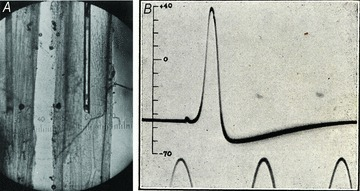
\includegraphics[width=0.5\textwidth]{ActionPotential.jpg}
\caption[Esperimento di \cite{Hodgkin1952}]
{ Sonda e misurazione del potenziale d'azione nell'assone del calamaro gigante {\it Loligo forbesi} nell'esperimento di \cite{Hodgkin1952}. In \cite{Schwiening2012}. }
\label{fig:ActionPotential}
\end{figure}


\begin{equation}
 I = C\frac{dV}{dt} + a_{K}(V-V_{K}) + a_{Na}(V-V_{Na}) + a_{l}(V-V_{l})
\end{equation}




%-----------------------------------------------------------------------
\section{La tecnologia di rilevazione CMOS-MEA}
\label{sez:Mea}\label{sez:Rilevazione}

{\it Micro Array Technology}. Si tratta di una tecnica di rilevazione e di stimolazione basata su un rivelatore piano composto di micro elettrodi utilizzata per la prima volta nel 1972 in ambito medico. Le cellule neuronali coltivate in vitro aderiscono alla superficie del rilevatore dove in prossimità degli elettrodi è sensibile al potenziale d'azione (scariche ioniche extracellulari, cfr. \ref{sez:Potenziale} ) ed è capace anche di fornire un segnale elettrico di stimolazione.

\begin{figure}%[tbp] 
\centering    
\includegraphics[width=0.5\textwidth]{Mea.png}
\caption[Rivelatore MEA]
{ (a) Layout MEA. (b) Schema microelettrodi e aperture. (c,d) MEA con coltura di cellule in una cilindro di vetro aperto sul fondo.  \cite{Kim2014}. }
\label{fig:MEA}
\end{figure}

Parametri critici dei rivelatori MEA sono la densità e l'impedenza dei micro elettrodi. I valori tipici per questi due parametri sono riportati nella tabella \ref{tab:DimensionamentoMea}.

\paragraph{Impedenza} L'impedenza dei microelettrodi dipende dalla loro area che può essere aumentata con la formazione di nanostrutture metalliche come nanotubi o nanopori che aumentano le capacità di rivelazione dei sensori \cite{Kim2014}.

\paragraph{Densità} La densità spaziale deli elettrodi nel sensore MEA può essere drasticamente aumentata con transistor CMOS integrati in un chip\footnote{Il cui disegno è effettuato con tecniche
VLSI {Very Large Scale Integration}, atte a implementare nello stesso chip di rivelazione anche i circuiti di amplificazione, multiplexing, conversione analogico-digitale e filtro}.

\begin{table}%[c]
\begin{tabular}{l|c|c|c}
{\bf Elettrodi}             & MEA                & CMOS-MEA   & NeuroChip \\ \hline

Numero                   & 512 & 16.384 & 98.304    \\
Diametro ($\mu m$)       & 20  & 20     & 5         \\
Spaziatura ($\mu m$)     & nr  & 20     & 5         \\
Rumore ($\mu V_{rms}$)   & 50  & 2.4    & 80-120    \\
Impedenza a 1$kHz$, ($k\Omega$)
                         & 30  & nr     & nr \\ 
SNR per elettrodo (dB)   & 100 & nr     & 3-7 \\
Potenza richiesta ($mW$) &  nr & 135    & nr \\
\hline
\end{tabular}
\caption[Dimensionamenti tipici MEA]
{Tecnologia MEA. Dimensionamenti tipici. Dati da \cite{Kim2014, Vallicelli2017}}
\label{tab:DimensionamentoMea}
\end{table}



%-----------------------------------------------------------------------
\section{L'algoritmo di spike sorting nell'esperimento Neuro Chip}
\label{sez:NeuroChip}

Attraverso la tecnologia presentata nelle sezioni precedenti, l'esperimento Neuro Chip riceve un segnale complesso composto da picchi di potenziale d'azione, caratterizzati approssimativamente da ampiezze di $500$ $mV$ e frequenze nell'ordine dei $kHz$, sovrapposto ad un segnale rumoroso derivante sia dalla componente tecnologica che quella biologica. L'entità del rumore varia dai $5-7dB$ $SNR$.  Fin qui l'organizzazione spaziale dei rilevatori CMOS è stata trascurata, laddove invece ognuno dei $16x192$ pixel è in grado di generare un segnale indipendente registrato ad altissima frequenza in modo da poter trattare contemporanei i segnali da pixel diversi.

L'alta risoluzione spaziale e temporale del sensore fa si che un singolo picco di potenziale sia rilevato contemporaneamente da un array di $3x3$ sensori per un intervallo temporale della durata di $3$ campioni consecutivi. Sulla base di questa sistematicità la rilevazione di un picco è basata su un test statistico del $Chi2$, in base al quale una porzione di segnale contiene un picco se la media quadratica normalizzata per la varianza del segnale è superiore ad un dato valore di soglia.

\begin{equation}
 \sum_{i,j=1,2,3} \sum_{t=0}^{2} \frac{|V_{i,j}(t)|^{2}}{\sigma_{i,j}^{2}} \geq \tau
\end{equation}

La soglia $\tau$ in un test statistico è determinata dalla dall'ampiezza desiserata del test secondo l'impostazione di Neyman e Fischer. Sulla base del contributo di \cite{Lambacher2011} nell'esperimento Neurochip, la soglia $\tau$ è determinata sperimentalmente in sede di calibrazione della strumentazione.

\begin{figure}%[tbp] 
\centering    
\includegraphics[width=0.5\textwidth]{Pixel.png}
\caption[Schema pixel esperimento Neuro chip]
{ Schema pixel esperimento Neuro chip.
Da \cite{Vallicelli2017}. }
\label{fig:Pixel}
\end{figure}

%% !TEX root = ../toptesi-scudo-example.tex
% !TEX encoding = UTF-8 Unicode
%***********************************************************************
%*********************************** First Chapter 

%***********************************************************************
%\cite{lamport1994latex, hertel2010writing}.
%Please see appendix~\ref{Appendix1}.
%***********************************************************************

\chapter{Costruzione di un filtro per segnali a tempo discreto}
\label{segnali}

\graphicspath{{Graph/}}

In questo capitolo si riportano le principali nozioni di teoria dei segnali utilizzate per l'analisi e l'implementazione del filtro. Le referenze utilizzate sono \cite{Oppenheim1998} per la teoria e le dimostrazioni riguardanti la funzione di risposta agli impulsi e l'analisi spettrale del segnale. Il testo di 
\cite{Diniz2010} è stato invece consultato per quanto riguarda gli esempi e le applicazioni con le librerie matlab già disponibili.



%-----------------------------------------------------------------------
\section{Rappresentazione convoluzionale}

Un segnale a tempo discreto è una successione di valori reali $x:=(x_{n})_{n\in Z}$. Il segnale può essere intrinsecamente discreto o frutto di un campionamento da un segnale continuo $x_{n} = x(nT_{s})$, dove $T_{s}^{-1} = \nu_{s}$ è la frequenza di campionamento. Nell'analisi dei segnali a tempo discreto riveste particolare rilievo la scrittura $x_{n} = \sum_{m} x_{m}\delta_{n-m}$, della successione in termini di somma convoluzionale con un treno di impulsi, dove $\delta_{n-m}=1$ se $n=m$ e $0$ altrimenti. Se $*$ indica l'operazione di somma di convoluzione $x*y = \sum x_{m}y_{n-m} = \sum y_{m}x_{n-m} = y*x$, si può scrivere anche $x=x*\delta$.

Una classe importante di operatori sui segnali discreti sono quelli lineari, ovvero tali che $ T(ax+by) = aT(x)+bT(y) $ ed omogenei, che commutano cioè con l'operatore di traslazione. Se $ S_{a}x = x_{-a}$ $x_{n}\rightarrow x_{n-a}$, allora affinché l'operatore $T$ sia omogeneo dovrà verificarsi che $TS_{a} = S_{a}T$. In tale classe, ad ogni operatore è associato un segnale detto di risposta agli impulsi che si indicherà con $h_{n}$. Posto$T(x)=y$ e $T(\delta) = h$ allora $T(x_{n}) = y_{n} = \sum x_{m}h_{n-m}$, dove $T(\delta_{n-m}) = h_{n-m}$, per cui $y=x*h$. Tutti gli operatori lineari e omogenei sono perciò descritti da una somma di convoluzione, la cui successione di risposta agli impulsi $h$ caratterizza l'operatore $T$.

In questi termini, per le proprietà di $*$, due trasformazioni in serie $T_{1}T_{2}$ sono rappresentate da $h_{1}*h_{2} = h_{2}*h_{1}$ e due trasformazioni in parallelo $T_{1} + T_{2}$ da $h_{1} + h_{2}$.



\section{Funzione di risposta agli impulsi. Trasformata z}
Dalla sezione precedente, una generica trasformazione lineare ed omogenea di un segnale di input $x:=(x_{n})_{n\in Z}$ in un segnale di output
$y:=(y_{n})_{n\in Z}$ si può scrivere in termini della somma di convoluzione
\begin{equation}
 y_{n} = \sum x_{m}h_{n-m} = \sum h_{m}x_{n-m}
\end{equation}
dove $h$ prende il nome di funzione di risposta agli impulsi e contiene tutta l'informazione necessaria per caratterizzare la trasformazione da $x$ a $y$. 

La rappresentazione convoluzionale fornita in termini di $h$ della trasformazione dimostra i suoi vantaggi nel momento in cui si trasforma un segnale in una funzione olomorfa attraverso la trasformata z, che ad un segnale $x$ associa, la funzione $X(z) = \sum x_{n}z^{n}$, $z\in C$, posto che si abbia convergenza in una regione connessa del piano complesso.

Dalla definzione di trasformata z si verifica che
\begin{equation}
 Y(z) = H(z)X(z)
\end{equation}
lo studio della funzione complessa $H(z)$, nel modulo e nella fase, risulta chiaramente più agevole di quanto in genere sia possibile con la successione di risposta gli impulsi $h$.

La funzione $H(z)$ inoltre, qualora il dominio di convergenza includa il cerchio unitario del piano complesso si riduce alla trasformata di Fourier del segnale
una volta che si pone $z = e^{iw}$.



%-----------------------------------------------------------------------
\section{Analisi spettrale di un segnale}

Attraverso la trasformata di Fourier discreta, ad un segnale finito di $N$ campioni $(x_{n})_{n=0,1,...N-1}$ è sempre possibile assegnare uno spettro discreto $(X_{k})_{k=0,1,...N-1}$ l'intepretazione del quale richiede di analizzare quali siano gli effetti del campionamento sullo spettro di Fourier di un ipotetico segnale continuo da cui quello finito è stato estratto. Le operazioni di estrazione qui di seguito analizzate sono:
\begin{itemize}
 \item Campionamento. $x(t)\rightarrow x(nT)$, $n\in Z$.
 \item Selezione o {\it windowing} $(x_{n})_{n\in Z} \rightarrow (x_{n})_{n=0}^{N-1} $
\end{itemize}



%-----------------------------------------------------------------------
\subsection{Campionamento di segnali continui}

Nel dominio del tempo il campionamento periodico
\footnote{Indicato nei diagrammi con la sigla $C/D$},
restituisce il segnale a tempo discreto $x_{n} = x(nT)$ dove $\nu = T^{-1}$ è la frequenza di campionamento. Per esplicitare gli effetti del campionamento nel dominio della frequenza risulta utile calcolare la trasformata di Fourier del segnale a tempo continuo
$ x_{s}(t) = x(t)s(t) $, che coincide con $x_{n}$ quando $t=nT$ ed è nullo altrove, e dove
$ s(t) = \sum_{n=-\infty}^{+\infty} \delta(t-nT_{s})$ è una sequenza di impulsi unitari. La trasformata di Fourier del segnale periodico $s(t)$ si può scrivere come sequenza di impulsi
\begin{equation}
S(jw) = \frac{2\pi}{T}\sum_{n=-\infty}^{+\infty} \delta(\frac{w}{T}-\frac{2\pi n}{T} ),
\end{equation}
da cui la trasformata di Fourier di $x_{s}(t)$ per convoluzione
$X_{s}(jw) = X_{c}(jw)*S(jw)$,
$X_{s}(jw) = \frac{1}{T} \sum_{n=-\infty}^{+\infty} X_{c}(j(\frac{w}{T}-\frac{2\pi n}{T}))$.
Lo stesso risultato si ottiene con la trasformata di Fourier di $x_{s}(t)$
\begin{align}
 & \int \sum_{n} x(t)\delta(t-nT)e^{j\Omega t} dt = \\
 & \sum_{n} x_{n} e^{-jw n} = \\
 & w \nu = \Omega.
\end{align}

Si conclude che data la trasformata di Fourier o spettro di un segnale a tempo continuo $X(j\Omega)$, lo spettro del segnale a tempo discreto $ X(e^{jw}) $ è una versione periodica e omotetica dello spettro continuo. Omotetia di costante pari alla frequenza di campionamento $\nu$.

\paragraph{Aliasing}
La periodicizzazione dello spettro continuo è causata dal campionamento. Due spettri successivi possono perciò sovrapporsi se la banda del segnale continuo è maggiore di due volte la frequenza di campionamento. Per evitare tale distorsione nello spettro discreto si prescrivono frequenze di campionamento superiori a due volte la massima frequenza del segnale continuo. Lo spettro continuo viene inoltre di solito sottoposto ad un filtro passa basso detto di anti aliasing che abbatte le frequenze superiori alla soglia desiderata.



%-----------------------------------------------------------------------
\subsection{Trasformata di Fourier discreta}
\label{sez:TDF}

Ad un segnale reale costituito da $N$ campioni $(x_{n})_{n=0}^{N-1}$ 
possono sempre essere associati i coefficienti della serie di Fourier del suo prolungamento per periodicità 
\begin{align}
 X_{SF}(k) & = \sum_{n=0}^{N-1} x_{n} e^{-j\frac{2\pi}{N}kn}  \\
 x_{n} &= \frac{1}{N} \sum_{k=0}^{N-1} x_{n} e^{j\frac{2\pi}{N}kn}
\end{align}
In questo senso il segnale $(x_{n})_{n=0}^{N-1}$ è inteso come la rilevazione di un solo periodo di durata $(N-1)T$, di un segnale periodico composto dall'infinita ripetizione del segnale osservato.
\footnote{Formalmente, il segnale periodico si può scrivere utilizzando l'operazione di modulo di due numeri interi
$x({mod}(n,N))$, $n\in Z$.}

Le frequenze campionarie $\frac{2\pi}{N}k$ utilizzate nelle espressioni precedenti sono quelle effettivamente osservabili in un campione finito. Infatti, preso ad esempio il segnale continuo
$x(t) = cos(\Omega t)$,
che campionato può essere scritto come
$x_{n} = cos( \frac{2\pi}{TN} k nT )$,
si verifica che le frequenze effettivamente osservabili sono
\begin{equation}
 \pm \pi \frac{2k}{N}, \quad k=0,...,\frac{N}{2}. 
\end{equation}
dove $k=0$ è la frequenza più bassa e $k=\frac{N}{2}$ la frequenza più alta.

La trasformata di Fourier di screta di un segnale finito di $N$ campioni è perciò composta da $N$ coefficienti della serie di Fourier $X_{SF}(k)$, $k = 0,... , N-1$.

Nel seguente esempio si esplicita la relazione della traformata discreta di Fourier e il campionamento di uno spettro del segnale continuo da cui sono state estratte le $N$ osservazioni.

Se $F(\Omega) = \int dt f(t)e^{-j\Omega t}$, ad esmepio per un segnale sinusoidale,
$F(\Omega) = \frac{A_{0}}{2}(\delta(\Omega-\Omega_{0}) + \delta(\Omega+\Omega_{0}))$
l'osservazione di una finestra di durata $(N-1)T$ ha effetto nello spettro
\begin{align}
V & = F*W = \frac{1}{2\pi} \int d\Theta F(\Theta) W(\Omega - \Theta)    \\
V(\Omega ) & = \frac{A_{0}}{2\pi}\frac{1}{\Omega - \Omega_{0}}
e^{j(\Omega-\Omega_{0})\frac{N-1}{2}} sen( (\Omega-\Omega_{0}) \frac{N-1}{2} ) + ...
\end{align}

Se lo spettro viene campionato alle frequenze empiriche $\frac{2\pi}{N} k$, $k=0,..., N-1$

\begin{equation}
\frac{1}{T}V(\frac{2\pi}{N}n) = \frac{A_{0}}{2\pi}\frac{1}{ w-w_{0} }
e^{j(w-w_{0})\frac{N-1}{2}} sen( (w-w_{0}) \frac{N-1}{2} ) + ...
\end{equation}

Si verifica che

\begin{equation}
\frac{1}{T} V(\frac{2\pi}{NT}k) = X_{FS}(k).
\end{equation}



%-----------------------------------------------------------------------
\subsection{Windowing}

In concreto il segnale reale si può ottenere moltiplicando il segnale a tempo discreto per una finestra $w_{n}=1$ se $n=0,1,...,N-1$ e $0$ altrove. Per cui il segnale osservato si può scrivere in forma di prodotto
$v_{n} = x_{n}w_{n}$, $n\in Z$
e la trasformata di Fourier in forma di convoluzione
$V = X*W$, dove $W(jw) = \sum_{n=0}^{N-1} e^{jwn}$ è calcolata in \ref{DIM_W}.
L'effetto di $W$ sullo spettro $X$ è sia sulle frequenze che sulle ampiezze e dipende in larga parte dalla forma della funzione $W$ i cui parametri principali sono l'altezza all'origine $|W(0)| = N$ e la base del picco all'ordine zero
$w_{0} = \pm\frac{2\pi}{L}$, $W(w_{0}) = 0$.


\begin{figure}[tbp] 
\centering    
\includegraphics[width=0.8\textwidth]{c2s0Window.eps}
\caption{Finestra quadrata nel dominio delle frequenze. $N=$ 1024, $\nu=$ 9kSAMPLES/s.}
\label{fig:c2s0Window}
\end{figure}




%-----------------------------------------------------------------------
\section{Disegno di un filtro in frequenza}

Un filtro la cui funzione di trasferimento ha fase nulla e modulo pari ad una finestra che seleziona una determinata banda di frequenze con precisione infinita si dice ideale e per essere implementato necessita di tutti i valori del segnale. Secondo la definizione data in \ref{}
il sistema risultante si dice non causale, in quanto i valori della sequenza filtrata in un determinato momento dipendono anche dai valori del segnale di input successivi. Diversamente, si dice causale un sistema dove la sequenza filtrata può essere calcolata in tempo reale, perchè il filtro è una funzione di soli valori passati della sequenza di input e della sequenza filtrata.
I sistemi ricorsivi come quelli descritti da equazioni alle differenze lineari del tipo
\begin{equation}
\sum_{l=0}^{L} y_{n-l}a_{l} = \sum_{m=0}^{M} x_{n-m}b_{m}
\label{eq:EDF}
\end{equation}
sono un esempio di sistemi causali facilmente implementabili e ampiamente utilizzati di cui fa parte il filtro analizzato in questo lavoro

La  funzione di trasferimento del sistema \ref{eq:EDF} nel piano-z è data una funzione razionale di polinomi in $z$
\begin{equation}
 H(z) = \frac{ \sum_{l=0}^{L} z_{-l}a_{l} }
             { \sum_{m=0}^{M} z_{-m}b_{m} },
\label{eq:Hz}
\end{equation}
che può essere riscritta in modo da evidenziare poli, zeri e relativi ordini.
\begin{equation}
 H(z) = \frac{ \prod_{k=1}^{Z} (1-z_{k}z^{-1}) }
             { \prod_{k=1}^{P} (1-p_{k}z^{-1}) }.
\label{eq:Hzp}
\end{equation}
La prima rappresentazione \ref{eq:Hz} ha un'immediata lettura dei coefficienti dell'equazione \ref{eq:EDF}, la seconda trova utilizzo nell'analisi delle proprietà del filtro.

Nel seguente grafico \ref{fig:c2s0MagPhase} si riportano l'attenuazione in ampiezza del filtro utilizzato e la distorsione di fase in termini di frequenze normalizzate.

\begin{figure}%[tbp] 
\centering    
\includegraphics[width=0.9\textwidth]{c2s0MagPhase.eps}
\caption[Funzione di trasferimento del filtro]
{ Approssimazione di Butterworth filtro IIR, ordine 2, frequenza di stop a 350 Hz, 9 $kSAMPLES/s$. }
\label{fig:c2s0MagPhase}
\end{figure}


Il successivo grafico \ref{fig:c2s0ZeroPole} visualizza nel piano-z i parametri del filtro. 


\begin{figure}%[tbp] 
\centering    
\includegraphics[width=0.9\textwidth]{c2s0ZeroPole.eps}
\caption[Filtro nel piano-z: poli e zeri]
{ Approssimazione di Butterworth filtro IIR, ordine 2, frequenza di stop a 350 Hz, 9 $kSAMPLES/s$. }
\label{fig:c2s0ZeroPole}
\end{figure}




%-----------------------------------------------------------------------
\section{Implementazione di un filtro}

Con riferimento alla funzione di trasferimento di un filtro nel piano-z come quella dell'equazione \ref{eq:Hz}, i cui parametri $a_{k}$ e $b_{k}$, sono il frutto del disegno del filtro secondo le specifiche richieste, esistono diverse equazioni ricorsive, tutte matematicamente equivalenti, per la sua implementazione. Queste diverse formulazioni matematiche, tra loro equivalenti da un punto id vista formale, non lo sono però sotto il profilo implementativo. Trattandosi infatti di eseguire le operazioni elementari di somma e moltiplicazione su componenti elettronici a precisione finita, la precisa sequenza di operazioni può invece avere diverso impatto nell'affidabilità e nella velocità dei calcoli e nella complicazione dei circuiti necessari all'implementazione del filtro.

In questo lavoro si prendono in esame due diverse forme, note in letteratura come forma diretta I e II. La forma diretta I si ottiene dalle seguente operazioni
\begin{align}
Y     &= \frac{B(z^{-1})}{A(z_{-1})}X \\
Y     &= \frac{1}{A(z^{-1})}B(z^{-1})X    \\
y_{n} &= \sum_{1}^{N} a_{l}y_{n-l} + \sum_{0}^{M} b_{l}x_{n-l}.
\end{align}
La forma diretta II si ottiene
\begin{align}
Y     &=  B(z^{-1})\frac{1}{A(z_{-1})}X \\
W     &:= \frac{1}{A(z_{-1})}X        \\
Y     &= B(z^{-1})W \\
w_{n} &= \sum_{1}^{M} b_{l}w_{n-l} + x_{n},  \\
y_n   &= \sum_{1}^{N} a_{l}w_{n-l}. 
\end{align}
%
Le due forme differiscono per l'ordine in cui vengono implementati i poli e gli zeri della funzione di trasferimento. L'ordine può avere impatto sul risultato quando la precisione aritmetica è finita.
Una seconda importande differenza è che la forma diretta II usa solo i ritardi della variabile $w_{n}$, riducendo così il numero di componenti elettroniche preposte alla memorizzazione dei valori passati da tenere per il calcolo del filtro. Trattandosi della forma con il minor numero di ritardi necessari, la forma diretta II prende il nome di forma canonica.

In appendice \ref{appB:filtring} son riportati gli algoritmi matlab delle due forme, che con la precisione numerica disponile ad un comune pc, risultano chiaramente equivalenti. A fini di simulazione, la verifica dell'impatto dei due algoritmi dev'essere quindi verificata riducendo la precisione numerica utilizzata dal programma di calcolo usato.



%-----------------------------------------------------------------------
\section{Termini stocastici. Rumore}

Per tener conto di effetti non deterministici che si verificano nella rilevazione e nel trattamento dei segnali si utilizza generalmente un termine stocastico additivo nel segnale di input modelizzato per semplicità come un errore gaussiano di media nulla e varianza data. Il segnale risultante
$x_{n} + \epsilon_{n}$, dove $\epsilon_{n}$ è l'errore stocastico, può essere inteso come un processo stocastico di variabili aleatorie indipendenti ma non identicamente distribuite. Indipendenti perché lo sono $\epsilon_{n}$, e quindi non correlate, e non identicamente distribuite perché il valore atteso dipende dal valore di $x$ al tempo $n$, $<x_{n} + \epsilon_{n}> = x_{n}$.


%-----------------------------------------------------------------------
\subsection{Correlogramma e Periodogramma}
Per effetto della trasformazione $y_{n} = \sum x_{l}h_{n-l}$, il processo stocastico $y_{n}$ non è di variabili indipendenti e una misura della dipendenza lineare tra esse è data dal correlogramma $\phi(m)$ che misura l'autocorrelazione del processo $\phi(m) = <yy_{-m}>$.
Un risultato notevole riguarda gli spettri dei correlogrammi delle sequenze di input e output
\begin{equation}
 \Phi_{y}(e^{jw}) = |H(e^{jw})|^{2} \Phi_{y}(e^{jw}).
\end{equation}
Si verifica che l'area sotto lo spettro della trasformata di Fourier di un segnale è proporzionale alla potenza totale del segnale ovvero alla varianza campionaria osservata, per cui l'effetto della funzione di trasferimento è quello di modulare la densità spettrale di potenza nelle frequenze di guadagno o attenuazione del filtro.

Nel caso del filtro analizzato in questo lavoro, ipotizzato un rumore di varianza $\sigma_{\epsilon}^{2}$ la modulazione della densità spettrale di potenza in dB è data da
\begin{equation}
10log_{10}(|H(e^{jw})|^2) + 20log_{10}(\sigma_{\epsilon}^{2}).
\end{equation}

\begin{figure}[tbp] 
\centering    
\includegraphics[width=0.9\textwidth]{c5s0Correlogram.eps}
\caption[Correlogramma di rumore bianco e densità spettrale di covarianza]
{ Correlogramma di rumore bianco e densità spettrale di covarianza. $
u$ 4,096kSAMPLES/s, $N$ 1024SAMPLES. SNR 0dB.}
\label{fig:Correlogram}
\end{figure}

%-----------------------------------------------------------------------
\subsection{Stima della densità spettrale di potenza}

Al cerscere dell'ampiezza campionaria la stima della densità spettrale di potenza diventa molto variabile. L'effetto è dovuto alla trasformazione di Fourier del correlogramma che ha ritardi molto elevati è calcolato con meno osservazioni. La variabilità sulla parte finale del correlogramma influisce su tutto lo spettro e quindi sulla stima della densità spettrale di potenza.

%% !TEX root = ../toptesi-scudo-example.tex
% !TEX encoding = UTF-8 Unicode
%**********************************************************************
%****************************** Third Chapter 

% 3) Operatori lineari sullo spazio delle successioni
% Proprietà
% Causalità
% Invarianza rispetto a traslazioni temporali
% Risposta agli impulsi
% Operatori di convoluzione
% Trasformazioni di equazioni alle differenze
% Trasformata-Z
% Funzione di trasferimento e risposta in frequenza
% Trasformata di Fourier
% Rumore
% Potenza di densità spettrale
% Correlogramma e trasformata di Fourier

%**********************************************************************
\chapter{Operatori lineari sullo spazio delle successioni}
\label{chapter 3}
    \graphicspath{{Chapter3/}}

%****************************** First Section ****************
\section{Proprietà}
\label{section 3.1}

\subsection{Causalità}
\subsection{Invarianza rispetto a traslazioni temporali}
\subsection{Risposta agli impulsi}
\subsection{Operatore di convoluzione}

%****************************** Second Section ****************
\section{Trasformazioni di equazioni alle differenze}
\label{section 3.2}

\subsection{Trasformata Z}
\subsection{Funzione di trasferimento e risposta in frequenza}
\subsection{Trasformata di Fourier}

%****************************** Third Section ****************
\section{Rumore}
\label{section 3.3}

\subsection{Potenza di densità spettrale}
\subsection{Correlogramma e trasformata di Fourier}


%% !TEX root = ../toptesi-scudo-example.tex
% !TEX encoding = UTF-8 Unicode
%***********************************************************************
%*********************************** First Chapter 

%***********************************************************************
%\cite{lamport1994latex, hertel2010writing}.
%Please see appendix~\ref{Appendix1}.
%***********************************************************************

\chapter{Implementazione del filtro}
\label{cap:implementazione}

\graphicspath{{Graph/}}


\begin{figure}[tbp] 
\centering    
\includegraphics[width=1\textwidth]{c4s1g1.eps}
\caption[]
{ }
\label{fig:c4s0}
\end{figure}


\begin{figure}[tbp] 
\centering    
\includegraphics[width=1\textwidth]{c4s1g2.eps}
\caption[]
{ }
\label{fig:c4s0}
\end{figure}


\begin{figure}[tbp] 
\centering    
\includegraphics[width=1\textwidth]{c4s1g3.eps}
\caption[]
{ }
\label{fig:c4s0}
\end{figure}

%% !TEX root = ../toptesi-scudo-example.tex
% !TEX encoding = UTF-8 Unicode
%-----------------------------------------------------------------------


%-----------------------------------------------------------------------
\chapter{Implemetazione matlab}
\label{capitolo:matlab}
\graphicspath{{Graph/}}

In questo capitolo si verificano con simulazioni matlab le previsione teoriche del capitolo precedente. Grafici e valori vengono analizzati in particolare per verificare la correttezza dei fattori di normalizzazione e delle relazioni tra trasformata discreta di Fourier e spettro del segnale continuo con riferimento alla realizzazione di un semplice segnale sinusoidale. L'ampiezza campionaria e il tasso di campionamento sono stati stabiliti simili a quelli realizzabili nell'esperimento neuro chip.

La sezione conclude con l'implementazione del filtro, la verifica dell'abbattimento delle banda di spettro desiderata e il suo effetto nella densità spettrale di potenza del segnale con rumore di SNR simile a quello dell'esperimento neuro chip.



%-----------------------------------------------------------------------
\section{Spettro di un segnale di prova sinusoidale}

Partendo da un ipotetico segnale sinusoidale a tempo continuo di durata illimitata
\begin{equation}
s_{c}(t) = A_{0}cos(\Omega_{0}t + \theta_{0}) +A_{1}cos(\Omega_{1}t + \theta_{0}),\quad\quad -\infty< t < +\infty.
\end{equation}

Si effettua un campionamento alla frequenza di $\nu$ $SAMPLES/s$ di $N$ osservazioni utilizzando una finestra quadrata $w_{n}$ tra $0$ e $N-1$
\begin{align*}
s_{n}  &= A_{0}cos(\omega_{0}n + \theta_{0}) +A_{1}cos(\omega_{1}n + \theta_{0}),\quad\quad -\infty< n < +\infty,\\
2x_{n} &= 		  A_{0}w_{n}e^{j\theta_{0}+j\omega_{0}} + A_{0}w_{n}e^{-j\theta_{0}-j\omega_{0}} 
			+ A_{1}w_{n}e^{j\theta_{1}+j\omega_{1}} + A_{1}w_{n}e^{-j\theta_{1}-j\omega_{1}},    \\
x_{n} &= w_{n}s_{n}.
\end{align*}

Ottenendo così lo spettro
\begin{align*}
2X(e^{j\omega}) = 	  &A_{0}W(j(\omega-\omega_{0}))e^{j\theta_{0}} + A_{0}W(j(\omega+\omega_{0}))e^{-j\theta_{0}}  \\
			+ &A_{1}W(j(\omega-\omega_{1}))e^{j\theta_{1}} + A_{1}W(j(\omega+\omega_{1}))e^{-j\theta_{1}}
\end{align*}

Nel seguente grafico \ref{fig:c5s0FreqNoNoise} la trasformata di Fourier discreta viene mappata nelle frequenze del segnale continuo e scalata utilizzando la frequenza campionaria verifiando così le relazioni della sezione \ref{sez:TDF}.

Dal grafico si evincono anche le proprietà di simmetria della componente reale e immaginaria dello spettro discreto, nonchè l'effetto del windowing sull'ampiezza e la larghezza dei picchi.

\begin{figure}%[tbp] 
\centering    
\includegraphics[width=1\textwidth]{c5s0FreqNoNoise.eps}
\caption[Trasformata discreta di Fourier di un segnale sinusoidale]
{Segnale sinusoidale: $w_{-}=2\pi$262Hz, $w_{+}=2\pi$523Hz.
$\nu=$ 9kSAMPLES/s,$N=$ 1024 SAMPLES.}
\label{fig:c5s0FreqNoNoise}
\end{figure}

\newpage



%-----------------------------------------------------------------------
\section{Risoluzione spettrale}

Come previsto nella sezione \ref{sez:TDF}, la risoluzione spettrale può essere migliorata aumentando l'ampiezza campionaria.
Nel seguente grafico \ref{fig:c5s0FreqNoNoiseCloseFreq} si verifica la diminuzione della base dei picchi rispetto al grafico precendente e conseguente risoluzione di due picchi in frequenza molto vicini tra loro.

\begin{figure}%[tbp] 
\centering    
\includegraphics[width=1\textwidth]{c5s0FreqNoNoiseCloseFreq.eps}
\caption[Risoluzione spettrale]
{Segnale sinusoidale. $w_{-}=2\pi$515Hz, $w_{+}=2\pi$523Hz. $\nu=$ 9kSAMPLES/s,$N=$ 4096 SAMPLES.}
\label{fig:c5s0FreqNoNoiseCloseFreq}
\end{figure}

\newpage


%-----------------------------------------------------------------------
\section{Funzione di trasferimento del filtro}
\label{section trasferimento}

Coefficienti dell'approssimazione di Butterworth di un filtro passa alto alla frequenza di soglia di $500Hz$ al second'ordine. 

\begin{center}
\begin{tabular}[c]{cccccc}
A1 & A2 & A3 & B1 & B2 & B3\\
1 & -1.5134 & 0.6105 & 0.7810 & -1.5619 & 0.7810
\end{tabular}
\end{center}
\label{tab: parametri}


\pagebreak


%-----------------------------------------------------------------------
\section{Filtro dei dati}
\label{section filtro}


\begin{figure}%[tbp] 
\centering    
\includegraphics[width=1\textwidth]{c5s0FilteringNoNoise.eps}
\caption[Densità spettrale di potenza senza rumore]
{Segnale sinusoidale. $\omega_{-}=2\pi$262Hz, $\omega_{+}=2\pi$523Hz. $
\nu$ 9kSAMPLES/s,$N=$ 4096 SAMPLES.}
\label{fig:c5s0FilteringNoNoise}
\end{figure}


\newpage




%-----------------------------------------------------------------------
\section{Effetto del rumore}
\label{sez:FiltroRumore}


\begin{figure}%[tbp] 
\centering    
\includegraphics[width=1\textwidth]{c5s0FilteringNoise.eps}
\caption[Densità spettrale di potenza con rumore]
{Segnale sinusoidale. $\omega_{-}=2\pi$262Hz, $\omega_{+}=2\pi$523Hz. $
\nu$ 9kSAMPLES/s,$N=$ 4096 SAMPLES.SNR = 5 dB.}
\label{fig:c5s0FilteringNoise}
\end{figure}

\newpage



%-----------------------------------------------------------------------
\section{Effetto della PCA}
\label{sez:FiltroRumore}


%-----------------------------------------------------------------------
\subsection{Elevamento alla seconda potenza}

L'algoritmo di {\it spike sorting} prevede di trasformare il segnale con la trasformazione non lineare $x_{n}\rightarrow x_{n}{^2}$. Con riferimento ad un segnale sinusoidale di prova si verifica che l'effetto spettrale di tale trasformazione è molto sensibile alla presenza di un offset o di rumore nei dati.

Nel caso ideale di un segnale $x(t)=cos(\Omega_{0}t)$, l'elevamento alla seconda potenza porta ad un raddoppio della frequenza del segnale e all'aggiunta di una componente in continua
\begin{align}
 x(t)^{2} &= \frac{1}{4}( e^{j\Omega_{0}t} + e^{-j\Omega_{0}t} + 2)  \\
 X(e^{j\Omega}) &= \frac{1}{4}\delta(\Omega \pm \Omega_{0}) + 
 \frac{1}{2}\delta(\Omega)
\end{align}

In presenza di un offset $a$, le frequenze originarie rimangono nello spettro scalate per la costante di offset
\begin{align}
 (x(t)+a)^{2}   &= a^{2} + cos(\Omega_{0}t)^{2} + 2cos(\Omega_{0}t)  \\
 X(e^{j\Omega}) &= \frac{1}{4}\delta(\Omega \pm \Omega_{0}) + 
 a\delta(\Omega\pm\Omega_{0}) + (a^{2} + \frac{1}{2})\delta(\Omega)
\end{align}

In presenza di un termine di errore additivo
\begin{align}
 (x(t)+\epsilon(t))^{2} &= \epsilon(t)^{2} + cos(\Omega_{0}t)^{2} + 2\epsilon(t)cos(\Omega_{0}t)
 \end{align}
Il segnale medio ha uno spettro di offset uguale alla varianza del rumore.
Questo spiega la presenza di $5$ picchi nel primo grafico della figura \ref{fig:c5s0FilteringSquaredSignal}; anche con una piccola componente di rumore si verifica la presenza dei picchi di frequenza originali e del picco in conitua a causa della trasformazione $x_{n}\rightarrow x_{n}{^2}$.

Si osserva inoltre che nel caso con rumore, allo spettro si aggiunge quello del termine $2\epsilon(t)cos(\Omega_{0}t)$, di media nulla, ma che contribuisce sensibilmente al rumore del segnale.

\begin{figure}%[tbp] 
\centering    
\includegraphics[width=1\textwidth]{c5s0FilteringSquaredSignal.eps}
\caption[Effetto spettrale dell'elevamento a potenza 2 del segnale]
{Segnale sinusoidale. $\omega_{-}=2\pi$262Hz, $\omega_{+}=2\pi$523Hz. $
\nu$ 9kSAMPLES/s,$N=$ 4096 SAMPLES.SNR = 5 dB.}
\label{fig:c5s0FilteringSquaredSignal}
\end{figure}

\newpage



%-----------------------------------------------------------------------
\subsection{Media mobile di ordine 3}

La seconda operazione prevista dall'algoritmo di {\it spike sorting} è l'applicazione di una media mobile di ordine $3$ al segnale proveniente da un singolo pixel $ 3y_{n} = x_{n} + x_{n-1} + x_{n-2}$. L'effetto di smorzamento delle alte frequenze è visibile dal primo pannello nel grafico \ref{fig:c5s0FilteringNoiseFir.tex}. I pannelli successivi verificano che le frequenze intaccate da questa operazione sono solo quelle alte. 

L'operazione non ha perciò effetto sulla banda di frequenze interessate dal primo filtro. Questo si verifica anche se il segnale viene preventivamente elevato al quadrato. L'ultimo pannello del grafico \ref{fig:c5s0FilteringNoiseFir.tex} evidenzia infatti come la funzione di trasferimento complessiva della trasformazione composta segua, ad una prima analisi, l'andamento della funzione di trasferimento del filtro FIR 3 lungo tutto lo spettro.


\begin{figure}%[tbp] 
\centering    
\includegraphics[width=1\textwidth]{c5s0FilteringNoiseFir.eps}
\caption[Effetto spettrale del filtro Fir 3]
{}
\label{fig:c5s0FilteringNoiseFir.tex}
\end{figure}

\newpage


%-----------------------------------------------------------------------
\subsection{Algoritmo PCA}
\label{sez:algoritmoPCA}

Nelle due precedenti sezioni sono stati analizzati gli effetti generali sullo spettro complessivo delle trasformazioni di elevamento a potenza e di media mobile sul segnale originale. Al fine di verificare nel dettaglio l'effetto spettrale della composizione di queste due operazioni sulla banda delle basse frequenze in cui agisce anche il filtro passa alto di Butterworth, i seguenti grafici riportano un dettaglio delle trasformazioni subite dalla banda di interesse in un ventaglio di situazioni al variare dell'offset e del SNR del segnale.

\begin{figure}%[tbp] 
\centering    
\includegraphics[width=1\textwidth]{c5s0FilteringPCA.eps}
\caption[Effetto spettrale della PCA. Segnale senza rumore]
{Segnale sinusoidale. $\omega_{-}=2\pi$262Hz, $\omega_{+}=2\pi$523Hz. $
\nu$ 9kSAMPLES/s,$N=$ 4096 SAMPLES. HP = High pass filter. FIR3 = media mobile al terzo ritardo sul segnale filtrato HP. 2FIR3 = media mobile al terzo ritardo sul segnale filtrato HP al quadrato. }
\label{fig:c5s0FilteringPCA}
\end{figure}

In questo primo grafico \ref{fig:c5s0FilteringPCA} si verifica che anche con alto $SNR$, la componente di offset aggiunta dall'elevamento al quadrato del segnale ha poi un effetto di innalzamento delle frequenze vicine (quelle basse), con il risultato di annullare parzialmente l'effetto del filtro passa alto precedentemente applicato.
Dal confronto dei grafici \ref{fig:c5s0FilteringPCA} e \ref{fig:c5s0FilteringPCAOffset} si verifica che l'effetto di annullamento dle filtro HP è dovuto alla combinazione di elevamento alla seconda potenza del segnale e dal filtro FIR3. E tale effetto peggiora con l'abbassamento del $SNR$, come si verifica nel grafico \ref{fig:c5s0FilteringPCAOffset7Snr}.


\begin{figure}%[tbp] 
\centering    
\includegraphics[width=1\textwidth]{c5s0FilteringPCAOffset.eps}
\caption[Effetto spettrale della PCA. Offset]
{HP = High pass filter. FIR3 = media mobile al terzo ritardo sul segnale filtrato HP. 2FIR3 = media mobile al terzo ritardo sul segnale filtrato HP al quadrato. }
\label{fig:c5s0FilteringPCAOffset}
\end{figure}


\begin{figure}%[tbp] 
\centering    
\includegraphics[width=1\textwidth]{c5s0FilteringPCAOffset7Snr.eps}
\caption[Effetto spettrale della PCA. Offset e SNR 7]
{HP = High pass filter. FIR3 = media mobile al terzo ritardo sul segnale filtrato HP. 2FIR3 = media mobile al terzo ritardo sul segnale filtrato HP al quadrato. }
\label{fig:c5s0FilteringPCAOffset7Snr}
\end{figure}


% !TEX root = ../toptesi-scudo-example.tex
% !TEX encoding = UTF-8 Unicode
%-----------------------------------------------------------------------


%-----------------------------------------------------------------------
\chapter{Logica di simulazione}
\label{capitolo:logica}
\graphicspath{{Graph/}}




In questa sezione due algoritmi di rilevazione degli impulsi sono messi a confronto su dei segnali di prova. L'analisi della capacità di discriminazione degli impulsi è condotta lungo i profili temporale e spettrale.


\paragraph{Profilo temporale.}
Sotto il profilo temporale, si verifica la corretta previsione del momento in cui si verifica un impulso. La metrica naturale di qualità dell'algoritmo sotto questo profilo dipende dal numero di falsi positivi e falsi negativi sul totale di impulsi nel segnale di prova. Adottando un criterio di soglia per l'identificazione di un impulso, $t=t_{spike} \Leftrightarrow V(t)>V_{soglia}$, la capacità discriminante dell'algoritmo dipende in ultima analisi dal guadagno differenziale tra le frequenze degli impulsi e quelle del rumore ed è perciò strettamente connessa al profilo spettrale.


\paragraph{Profilo spettrale.}
Sotto il profilo spettrale l'analisi riguarda la forma dello spettro dopo le trasformazioni previste dall'algoritmo di rilevazione. La metrica sarà un'opportuna distanza tra lo spettro ideale e quello risultante dall'algoritmo, eventualmente ristretta alla banda di frequenze di interesse.


\subparagraph{Spettro di riferimento.}
Per {\it spettro ideale} si intende lo spettro che si otterrebbe campionando il segnale proveniente da un singolo pixel, contenente un unico impulso, a parità di durata e tasso di campionameno, e senza rumore, o più realisticamente, con un $SNR$ molto alto.






%-----------------------------------------------------------------------
\section{Algoritmo di rilevazione a media semplice}

Dopo aver applicato un filtro passa banda singolarmente ai segnali di ogni pixel del cluster, si ottiene un segnale medio applicando una media semplice.
In formule, con $y_{k, n, j}$ il segnale, dove $k=1, 2, 3, 4$ è l'indice dello stadio della trasformazione, $n$ il campione al tempo $n/\nu_{sampling}$ e $ j=1, .., N $ l'indice del pixel nel cluster.

\begin{align*}
y_{1, n, j } & = a_{0}y_{1, n, j } + a_{1}y_{1, n-1, j } + b_{0}x_{n} + b_{1}x_{n-1} + b_{2}x_{n-2}  &\quad\mathtt{band pass step}\\
y_{2, n    } & = \frac{\sum_{j=1}^{N} y_{1, n, j }}{N}  &\quad\mathtt{spatial average step}\\
\end{align*}



%-----------------------------------------------------------------------
\section{Algoritmo di rilevazione a media quadratica}

Dopo aver applicato un filtro passa banda singolarmente ai segnali di ogni pixel del cluster, si ottiene un segnale medio del cluster con una media quadratica. Al segnale quadratico medio viene dopodiché applicato un filtro a media mobile di ordine 3.

In formule, con $y_{k, n, j}$, dove $k=1, 2, 3, 4$ è l'indice dello stadio della trasformazione, $n$ il campional tempo $n/\nu_{sampling}$ e $j=1, .., N$ l'indice del pixel.

\begin{align*}
y_{1, n, j } & = a_{0}y_{1, n, j } + a_{1}y_{1, n-1, j } + b_{0}x_{n} + b_{1}x_{n-1} + b_{2}x_{n-2}  \\
y_{2, n, j } & = y_{1, n,j}^{2}   \\
y_{3, n    } & = \sum_{j=1}^{N} y_{2, n, j } / N    &\quad\mathtt{spatial average step}\\
y_{4, n    } & = \sum_{t=0}^{3} y_{3, n-t } / 3 &\quad\mathtt{moving average step}
\end{align*}



%-----------------------------------------------------------------------
\section{Logica di simulazione}

La simulazione introduce diversi tipi di incertezza nella rilevazione degli impulsi.

\paragraph{Tempo di interarrivo degli impulsi.}
La distribuzione degli impulsi è uniforme su tutto il segnale. Fissato il numero totale di spike attesi in un campione di data lunghezza in base al parametro {\it spike rate}, gli impulsi sono uniformemente distribuiti in tutto il segnale. Si assume che il momento in cui viene rilevato lo spike sia uguale per tutti i pixel considerati.


\paragraph{Forma dell'impulso}
Si considerano forme di impulso diverse: rettangolare, gaussiana, gaussiana doppia e sinusoidale. Ciascuna ha durata di circa $1ms$ e picco massimo intorno a $60mV$ e sono tutte costruite in modo da trasferire la stessa potenza.


\paragraph{Fase di campionamento}
Ad ogni impulso e per ciascun pixel, la forma d'onda considerata viene campionata ad intervalli regolari da un punto di partenza variabile casualmente.
Con il tasso di campionamento a $\nu_{s}=9$ $kHz$ e la durata dell'impulso di circa $1ms$, si attendono circa 9 campioni su ciascun impulso. Data la forma di ciascun impulso si tiene conto di un possibile ritardo di campionamento (fase casuale) distribuito uniformemente nell'intervallo $\pm \nu_{s}^{-1} = \pm 1/9$ $ms$.


\paragraph{Rumore termico}
Rumore gaussiano di varianza stabilita in base all'$SNR$ fissato e alla potenza trasferito dall'impulso.
Si rimanda alla sezione \ref{{sez:calcoloSNR}} per un dettaglio del calcolo dell'$SNR$.





%-----------------------------------------------------------------------
\section{Parametri di simulazione}
\label{sez:parametri}



\begin{table}
\begin{center}
\begin{tabular}{l|c|c|c}
{\bf Parametro}             & Valore                & Unità \\ \hline

 & &     \\
Durata segnale             & 1      & s    \\
Tasso di campionamento     & 9      & kHz  \\
Tasso di spiking           & 5      & Hz   \\
Durata impulso             & 1-1.5  & ms   \\
Picco di potenziale AP     & 60     & mV   \\
SNR                        & 5-7    & dB   \\
                           &        &      \\
Ordine filtro passa banda  & 2      &      \\
 + pass band               & $>0.2$ & kHz  \\
 + stop band               & $>3$   & kHz  \\
                           &        &      \\
Pixel nel cluster          &    7   &      \\
 & &     \\
 
\hline
\end{tabular}
\caption[Parametri di simulazione]
{Parametri di simulazione}
\label{tab:paraemtri}
\end{center}
\end{table}







%-----------------------------------------------------------------------
\section{Forma degli impulsi e fase di campionamento}

I valori di riferimento degli impulsi neurali sono la durata di $1ms$ e il picco massimo di $60mV$. Non essendo nota la forma dell'impulso,  per semplicità, la simulazione considera come impulso base un periodo di un impulso in tensione sinusoidale
$ V(t) = (60mV) sin( wt) $, della durata di $1$ $ms$. Le altre forme di impulso sono dimensionate in modo tale da trasferire una potenza simile. L'esatta potenza di ciascun impulso viene poi utilizzata per il calcolo della varianza dell'errore termico in modo che simulazioni con impulsi diversi siano confrontabili in base all'$SNR$. Il seguente grafico \ref{fig:c6_impulseTable} riporta alcuni campionamenti dai diversi tipi di impuso considerati.

\begin{figure}%[tbp] 
\centering    
\includegraphics[width=1\textwidth]{c6_impulseTable.eps}
\caption[Forme degli impulsi]
{Forme degli impulsi.}
\label{fig:c6_impulseTable}
\end{figure}

\paragraph{Fase di campionamento}
Si verifica che al tasso di campionamento considerato, la fase di campionamento è una fonte di incertezza importante essendo più che grossolano il campionamento di un impulso della durata di $1ms$ con solo $9$ campioni. I seguenti grafici riportano con maggior dettaglio l'effetto della fase di campionamento.
\ref{fig:c6s0impulsoGauss}, \ref{fig:c6s0impulso2Gauss}.


\begin{figure}[tbp] 
\centering    
\includegraphics[width=0.6\textwidth]{c6s0impulsoGauss.eps}
\caption[Campionamento di un impulso gaussiano]
{3 campioni da un impulso gaussiano}
\label{fig:c6s0impulsoGauss}
\end{figure}


\begin{figure}[tbp] 
\centering    
\includegraphics[width=0.6\textwidth]{c6s0impulso2Gauss.eps}
\caption[Campionamento di due impulsi gaussiani]
{3 campioni da due impulsi gaussiani}
\label{fig:c6s0impulso2Gauss}
\end{figure}






%-----------------------------------------------------------------------
\section{Calcolo potenza di rumore per dato SNR}
\label{sez:calcoloSNR}

L'impulso di riferimento per la simulazione è quello sinusoidale.
La tabella \ref{tab:impulsi} specifica la parametrizzazione utilizzata e riporta i valori di potenza e durata degli impulsi in modo tale che forme di impulso diverse abbiano la stessa potenza di quello sinusoidale di picco $V_{0}$ a $60$ $mV$ e durata $1ms$, ovvero $1,8$ $\mu V^{2}s$.


\begin{table}%[tbp]
\begin{tabular}{l|c|c|c|c|}
{\bf Impulso}   & Potenza &  & Durata &  \\ \hline

& & & &     \\

$S(t)  = V_{0}sin(\Omega t)$
&   & 
& 1 periodo  &  - \\

$S(\Omega)^{2}  = V_{0}^{2}\delta(\pm \Omega - \Omega_{0})$
&  $V_{0}^{2}\frac{L}{2}$ & $1,8$ $\mu V^{2}s$
& $L$ &  $1ms$ \\   \hline


$V(t) = V_{0}e^{-\frac{t^2}{A^2}}$
&  %$V_{0}A\sqrt{\pi}$ 
& 
& $\frac{3}{\sqrt{2}}A$ & $1$ $ms$    \\

& & & &     \\

$V(\Omega)^{2} = V_{0}^{2}\frac{A^{2}}{2}e^{-\frac{\Omega^{2}A^{2}}{2}}$
&  $V_{0}^{2}A\sqrt{\frac{\pi}{2}}$ & $2.127$ $(mV)^{2}ms$
& $\frac{3}{A}$ &  $6.36$ $kHz$   \\   \hline

& & & &     \\

$R(t) = V_{0}\chi(\pm \frac{b}{2})$
&  %$V_{0}b$ 
& $60$ $mV$
& $b$ &  $0.59$ $s$  \\

& & & &     \\

$R(t)^{2}  = V_{0}^{2}\chi(\pm \frac{b}{2})$
&  $V_{0}^{2}b$ & $1,8$ $\mu V^{2}s$
& $b$ &  - \\

\hline

\end{tabular}
\caption[Impulsi: potenza e durata]
{Impulsi: potenza e durata}
\label{tab:impulsi}
\end{table}


La potenza di rumore utilizzata per dato $SNR$ è stata calcolata tenendo conto della potenza trasferita nel tempo di durata di un singolo impulso, secondo le seguenti relazioni.

\begin{align*}
P_{noise} \quad [V^2s] &=  P_{impulse} 10^{- snr [dB]/10} \\
\sigma^2 &= \frac{ P_{noise} }{ \nu_{s} T_{s} }\\
\epsilon_{n} &\sim norm(0,\sigma^2) 
\end{align*}

dove $\nu_{s} $ è il tasso di campionamento e $ T_{s} $ la durata dell'impulso; $\sigma$ è la deviazione standard dell'errore additivo aggiunto al segnale in ogni campionamento. Con riferimento all'impulso di riferimento sinusoidale, il seguente grafico \ref{fig:c6_graphSNR} riporta le deviazioni standard utilizzate in funzione dell'SNR.


% function genGraphSigmaSNR(p)
\begin{figure}%[tbp] 
\centering    
\includegraphics[width=0.8\textwidth]{c6_graphSNR.eps}
\caption[Calcolo potenza di rumore.]
{Calcolo potenza di rumore.}
\label{fig:c6_graphSNR}
\end{figure}






%-----------------------------------------------------------------------
\chapter{Risultati}
\label{capitolo:risultati}
\graphicspath{{Graph/}}



%-----------------------------------------------------------------------
\section{Algoritmo quadratico}

I grafici riportano nella prima colonna il segnale nel dominio del tempo e della frequenza e nella colonna a destra il segnale filtrato con l'algoritmo di rilevazione degli impulsi. Gli asterischi rossi indicano i momenti in cui sono stati simulati gli impulsi.

Lo {\it spettro di riferimento} è lo spettro che si otterrebbe campionando con lo stesso tasso di campionameno un segnale della stessa durata con un solo impulso, senza rumore o più realisticamente, con un $SNR$ alto.


\begin{figure}[tbp] 
\centering    
\includegraphics{c6_I2T2SNR-39Simulazione.eps}
\caption[Algoritmo media quad. Impulso $2$. $SNR=-39$.]
{Algoritmo media quad. Impulso $2$. $SNR=-39$.}
\label{fig:c6_I2T2SNR-32Simulazione}
\end{figure}


\begin{figure}[tbp] 
\centering    
\includegraphics{c6_I3T2SNR-40Simulazione.eps}
\caption[Algoritmo media quad. Impulso $3$. $SNR=-40$.]
{Algoritmo media quad. Impulso $3$. $SNR=-40$.}
\label{fig:c6_I3T2SNR-40Simulazione}
\end{figure}


\begin{figure}[tbp] 
\centering
\includegraphics{c6_I4T2SNR-41Simulazione.eps}
\caption[Algoritmo media quad. Impulso $4$. $SNR=-41$.]
{Algoritmo media quad. Impulso $4$. $SNR=-41$.}
\label{fig:c6_I4T2SNR-41Simulazione}
\end{figure}


\begin{figure}[tbp] 
\centering    
\includegraphics{c6_I5T2SNR-43Simulazione.eps}
\caption[Algoritmo media quad. Impulso $5$. $SNR=-43$.]
{Algoritmo media quad. Impulso $5$. $SNR=-43$.}
\label{fig:c6_I5T2SNR-43Simulazione}
\end{figure}



\pagebreak




%-----------------------------------------------------------------------
\section{Algoritmo in media semplice}

I grafici riportano nella prima colonna il segnale nel dominio del tempo e della frequenza e nella colonna a destra il segnale filtrato con l'algoritmo di rilevazione degli impulsi. Gli asterischi rossi indicano i momenti in cui sono stati simulati gli impulsi.

Lo {\it spettro di riferimento} è lo spettro che si otterrebbe campionando con lo stesso tasso di campionameno un segnale della stessa durata con un solo impulso, senza rumore o più realisticamente, con un $SNR$ alto.


\begin{figure}[tbp] 
\centering    
\includegraphics{c6_I2T1SNR-39Simulazione.eps}
\caption[Algoritmo media semplice. Impulso $2$. $SNR=-39$.]
{Algoritmo media quad. Impulso $2$. $SNR=-39$.}
\label{fig:c6_I2T1SNR-32Simulazione}
\end{figure}


\begin{figure}[tbp] 
\centering    
\includegraphics{c6_I3T1SNR-40Simulazione.eps}
\caption[Algoritmo media semplice. Impulso $3$. $SNR=-40$.]
{Algoritmo media quad. Impulso $3$. $SNR=-40$.}
\label{fig:c6_I3T1SNR-40Simulazione}
\end{figure}


\begin{figure}[tbp] 
\centering    
\includegraphics{c6_I4T1SNR-41Simulazione.eps}
\caption[Algoritmo media semplice. Impulso $4$. $SNR=-41$.]
{Algoritmo media quad. Impulso $4$. $SNR=-41$.}
\label{fig:c6_I4T1SNR-41Simulazione}
\end{figure}


\begin{figure}[tbp] 
\centering    
\includegraphics{c6_I5T1SNR-43Simulazione.eps}
\caption[Algoritmo media semplice. Impulso $5$. $SNR=-43$.]
{Algoritmo media quad. Impulso $5$. $SNR=-43$.}
\label{fig:c6_I5T1SNR-43Simulazione}
\end{figure}


\pagebreak




%-----------------------------------------------------------------------
\section{Risultati: Distanza spettri}

Presa come metrica la distanza tra gli spettri

\begin{equation}
 d_{\nu_{1},\nu_{2}} = \| psd_{\nu_{1},\nu_{2}}^{*} - psd_{\nu_{1},\nu_{2}}^{f} - <psd_{*} - psd_{f}> \|_{2}
\end{equation}
\label{eqn:metrica}

dove $<psd_{*} - psd_{f}>$ è la media della differenza tra lo spettro ideale $psd_{*}$ e quello filtrato $psd_{f}$ complessivamente nell'intera banda, e $psd_{\nu_{1},\nu_{2}}^{*} - psd_{\nu_{1},\nu_{2}}^{f}$ la differenza degli spettri nella banda $(\nu_{1},\nu_{2})$, si verifica che gli l'algoritmi di sorting a media semplice restituiscono sempre spettri più vicino a quello ideale.


La tabella riporta la distanza tra lo spettro ideale e lo spettro ottenuto dopo le trasformazioni di quattro test. La distanza è calcolata sull'intera banda di frequenze.

Il test $1BP$ è il test a media semplice con un filtro passa banda $(BP)$ applicato a tutti i pixel prima della media.
Il test $2BP$ è il test a media quadratica con un filtro passa banda $(BP)$ applicato a tutti i pixel prima della media.
I test $1LP$ e $2LP$ corrispondono ai precedenti dove però il filtro è solo passa basso $LP$. Questi test sono stati introdotti per verificare se, per le forme di impuso a media positiva come quello gaussiano, la distorsione apportata dal filtro $BP$ sulle basse frequenze non comportasse un allontanamento apprezzabile degli spettri.

\begin{table}%[tbp]
\begin{center}
\begin{tabular}{|c|c|c|c|c|c|}

\hline
      & \multicolumn{5}{|c|}{Impulso}    \\
      \hline
Test  &  $1$  &  $2$ &   $3$ &   $4$ &   $5$ \\
      &       &      &       &       &       \\

  $1BP$  &  0.0010  &  0.0200 &   0.0195 &   0.0119 &   0.0165 \\
  &   &  &    &    &    \\
$2BP$  &  0.0020  &  1.1978 &   1.1909 &   1.2277 &   1.2332 \\
&   &  &    &    &    \\
$1LP$  &  0.0030  &  0.0192 &   0.0180 &   0.0117 &   0.0168 \\
&   &  &    &    &    \\
$2LP$  &  0.0040  &  1.2494 &   1.2500 &   1.2576 &   1.2331 \\
&   &  &    &    &    \\

         
         
\hline

\end{tabular}
\caption[Distanza dallo spettro ideale per tipo di sorting test e forma di impulso]
{Distanza dallo spettro ideale per tipo di sorting test e forma di impulso}
\label{tab:DFTdiff}
\end{center}
\end{table}







%-----------------------------------------------------------------------
\chapter{Conclusioni}
\label{capitolo:conclusioni}
\graphicspath{{Graph/}}


%-----------------------------------------------------------------------
\section{Conclusioni}


\paragraph{Distanza spettri.}


\paragraph{Andamento al variare del SNR}



\paragraph{Andamento al variare del tipo di impulso}



\paragraph{Effetto del filtro passa basso o passa banda}
Alcune forme di impulso come quelle a media non nulla, ad esempio il tipo $2$ gaussiano
ha uno spettro ideale che non diminuisce alle basse frequenze. Ha senso quindi applicare a priori un filtro passa banda? In questo caso le basse frequenze non costituiscono rumore ma sono parte del pacchetto di frequenze necessario a dar forma dell'impulso.

%% !TEX root = ../toptesi-scudo-example.tex
% !TEX encoding = UTF-8 Unicode
%-----------------------------------------------------------------------


%-----------------------------------------------------------------------
\chapter{Conclusioni e prospettive}
\label{capitolo:conclusioni}


\section{Campionamento discreto}

Nella ambito della teoria dei segnali sono ben note le trasfomazioni da operare allo spettro di un segnale continuo per giustifacare la trasformata discreta di Fourier di un segnale finito frutto del campionamento di quello continuo. In questo lavoro sono stati in particolar modo verificati e analizzati gli effetti del campionamento di una finestra quadrata di dati, con particolare riferimento alla risoluzione spettrale dei picchi di frequenza di un segnale di prova sinusoidale.

Sono note in letterature campionamente con finestre di dati non uniformi, che smorzando le osservazioni iniziali e finali del segnale ottengono risoluzioni spettrali migliori.


\section{Algoritmo di Implementazione}

I due algoritmi di impementazione qui analizzati non mostrano concrete differenze nella simulazione a causa dell'ampia disponibilità dei registri di memoria a precisione doppia utilizzati. Da una considerazione sul numero di operazioni richieste è noto che la forma {\it diretta 2} richiede l'uso di meno componenti elettronici dedicati ai ritardi del segnale di input e perciò è stata indicata come preferita.

Ulteriori verifiche dovrebbero essere condotte con simulazioni a precisione algebrica finita, per verificare le possibili fonti di rumore derivanti dal troncamento e la quantizzazione del segnale tipiche della fase di digitalizzazione.


\section{Effetto spettrale della PCA}

Nel grafico \ref{fig:c5s0FilteringPCA} si verifica che anche con alto SNR, la componente di offset aggiunta dall'elevamento al quadrato del segnale ha l'effetto di innalzare le frequenze vicine (quelle basse), con il risultato di annullare parzialmente l'effetto del filtro passa alto precedentemente applicato.
Dal confronto dei grafici \ref{fig:c5s0FilteringPCA} e \ref{fig:c5s0FilteringPCAOffset} si verifica che l'effetto di annullamento del filtro passa alto è dovuto alla composizione delle due operazioni della PCA; quella di elevamento alla seconda potenza del segnale e quella del filtro FIR3.

% Numbered appendices remain in the main matter...
% \appendix
% % !TEX root = ../toptesi-scudo-example.tex
% !TEX encoding = UTF-8 Unicode
% ******************************* Thesis Appendix A 

\chapter{Dimostrazioni}
\label{Appendix1}



%-----------------------------------------------------------------------
\section{Spettri notevoli}

\subsection{Finestra quadrata}
La successione $w_{n}=1$ per $n=0,1, ..., N-1$ e $0$ altrimenti, è stata applicata moltiplicativamente ad un segnale discreto $x_{n}$ per l'estrazione di un suo sotto campione di lunghezza finita, $y_{n} = w_{n}x_{n}$.
L'effetto sullo spettro di $x_{n}$ è dato dalla somma di convoluzione $ Y(e^jw) = W(e^jw)*X(e^jw) $, dove $ W(e^jw) $ si ottiene applicando la trasformata di Fourier a $w_{n}$.

\begin{align*}
w_{n} 		& = \sum_{m=0}^{N-1} \delta(n-m),	\\
W(e^{jw} ) 	& = \sum_{n=-\infty}^{+\infty} w_{n} e^{jwn} = \sum_{n=0}^{N-1} e^{jwn}.
\end{align*}

posto $z = e^jw $, la ragione della somma geometrica,
$\sum_{n=0}^{N-1} z^{n} = \frac{z^{N}-1}{z-1} = \frac{z^{N/2}}{z^{1/2}}\frac{z^{N/2}-z^{-N/2}}{z^{1/2}-z^{-1/2}} $
risulta che

\begin{align*}
W(e^{jw} ) 	& = e^{jw\frac{N-1}{2}}\frac{sen(w\frac{N}{2})}{sen(\frac{w}{2})}.
\end{align*}




% % !TEX root = ../toptesi-scudo-example.tex
% !TEX encoding = UTF-8 Unicode
% ******************************* Thesis Appendix B 

\lstloadlanguages{matlab}

\definecolor{mygreen}{rgb}{0,0.6,0}
\definecolor{mygray}{rgb}{0.5,0.5,0.5}
\definecolor{mymauve}{rgb}{0.58,0,0.82}

\lstset{ 
  backgroundcolor=\color{white},   % choose the background color; you must add \usepackage{color} or \usepackage{xcolor}; should come as last argument
  basicstyle=\footnotesize,        % the size of the fonts that are used for the code
  breakatwhitespace=false,         % sets if automatic breaks should only happen at whitespace
  breaklines=true,                 % sets automatic line breaking
  captionpos=b,                    % sets the caption-position to bottom
  commentstyle=\color{mygreen},    % comment style
  deletekeywords={...},            % if you want to delete keywords from the given language
  escapeinside={\%*}{*)},          % if you want to add LaTeX within your code
  extendedchars=true,              % lets you use non-ASCII characters; for 8-bits encodings only, does not work with UTF-8
  firstnumber=0,                % start line enumeration with line 1000
  frame=single,	                   % adds a frame around the code
  keepspaces=true,                 % keeps spaces in text, useful for keeping indentation of code (possibly needs columns=flexible)
  keywordstyle=\color{blue},       % keyword style
  language=Octave,                 % the language of the code
  morekeywords={*,...},            % if you want to add more keywords to the set
  numbers=left,                    % where to put the line-numbers; possible values are (none, left, right)
  numbersep=5pt,                   % how far the line-numbers are from the code
  numberstyle=\tiny\color{mygray}, % the style that is used for the line-numbers
  rulecolor=\color{white},         % if not set, the frame-color may be changed on line-breaks within not-black text (e.g. comments (green here))
  showspaces=false,                % show spaces everywhere adding particular underscores; it overrides 'showstringspaces'
  showstringspaces=false,          % underline spaces within strings only
  showtabs=false,                  % show tabs within strings adding particular underscores
  stepnumber=2,                    % the step between two line-numbers. If it's 1, each line will be numbered
  stringstyle=\color{mymauve},     % string literal style
  tabsize=2,	                   % sets default tabsize to 2 spaces
  %title=\lstname                   % show the filename of files included with \lstinputlisting; also try caption instead of title
}


%\begin{lstlisting}
%n = floor((N-1)/2);
%tf = exp(1i*pi*(1-1/N)*[0:n,n+1-N:-1]')*ones(1,nc) .* fft(f);
%tf = tf([n+2:N,1:n+1],:);
%\end{lstlisting}



\chapter{Codice sorgente}
\label{Appendix2}


\section{Trasformata discreta di Fourier simmetrica}
\lstinputlisting{/home/alfre/Documents/Unimib/Tesina/spikeFilter/matlab/filtering/sfft.m}


\section{Generazione segnale sinusoidale}
\lstinputlisting{/home/alfre/Documents/Unimib/Tesina/spikeFilter/matlab/filtering/mySignal.m}

\section{Implementazione del filtro}
\label{appB:filtring}
\lstinputlisting{/home/alfre/Documents/Unimib/Tesina/spikeFilter/matlab/filtering/myFiltering.m}
    



\backmatter% here begins the back matter
% ... otherwise a single appendix may stay here
\include{Biblio/biblio.bib}

% Do not use this command if you did not prepare a nomenclature
% database by means od the suitable \nomenclature command and its
% arguments, as we did in chapter 2 of this example thesis.
\printnomencl

% In this example we use \nocite{*} in order to typeset the whole
% contents of the bibliographic database. Normally this is not
% necessary and it's better to let biber extract from the database
% only the cited works
\nocite{*}


% \printbibliography[heading=bibintoc]

% Do not use this command if you did not set the \makeindex switch
% in the preamble.

\printindex

\end{document}

